\section{Evaluation}\seclabel{Evaluation}

implemented bpaxos, epaxos, and multipaxos in scala

\subsection{Latency and Throughput}
{\begin{figure*}[ht]
  \centering
  \begin{subfigure}[c]{0.36\textwidth}
    \centering
    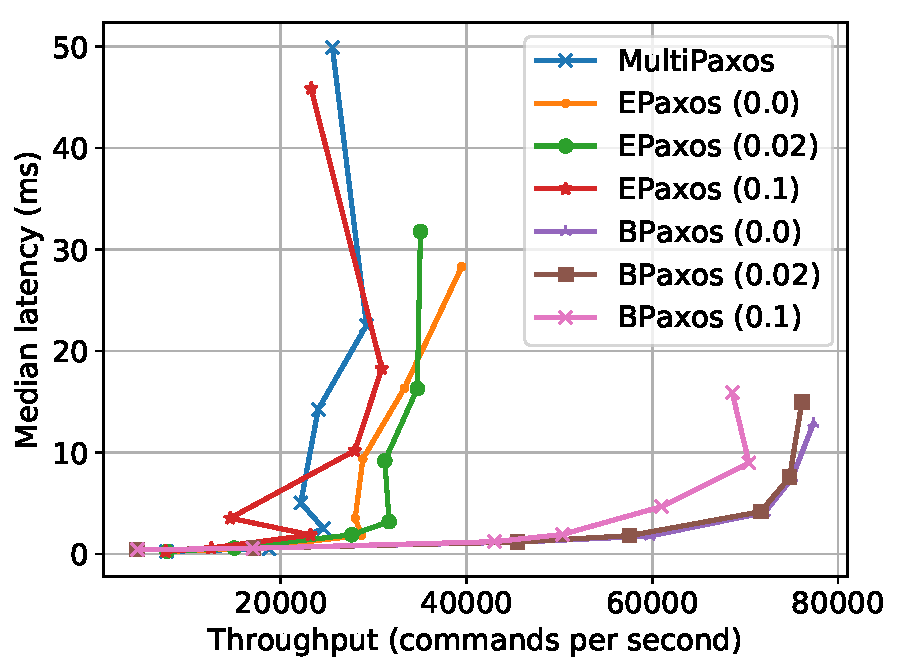
\includegraphics[width=\textwidth]{assets/nsdi_fig1_lt_f1.pdf}
    \caption{
      Latency-throughput curves for Multipaxos, EPaxos, and BPaxos. EPaxos and
      BPaxos are run with 0\%, 2\% and 10\% conflict rates. Here, $f = 1$.
    }\figlabel{EvalLtF1}
  \end{subfigure}
  \begin{subfigure}[c]{0.36\textwidth}
    \centering
    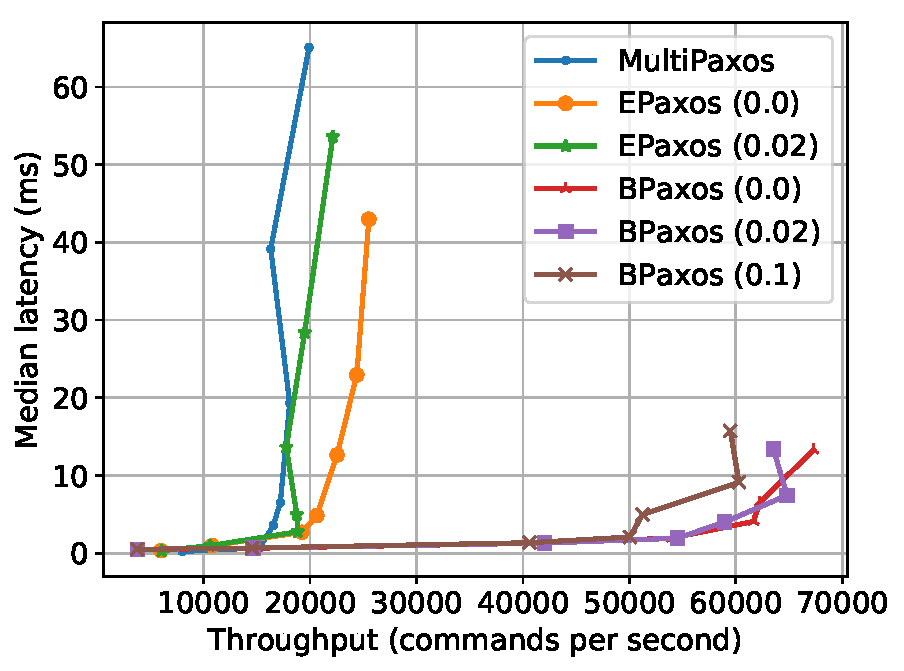
\includegraphics[width=\textwidth]{assets/nsdi_fig1_lt_f2.pdf}
    \caption{The same as \figref{EvalLtF1} but with $f=2$.}%
    \figlabel{EvalLtF2}
  \end{subfigure}
  \begin{subfigure}[c]{0.23\textwidth}
    \centering
    \small
    \begin{tabular}{lccc}
      \toprule
      \multicolumn{1}{c}{Protocol} &
      \multicolumn{3}{c}{Number of clients} \\
      %
                    & 1    & 10   & 50 \\\midrule
      Multipaxos    & 0.24 & 0.52 & 2.49 \\
      EPaxos (0.0)  & 0.25 & 0.56 & 1.83 \\
      EPaxos (0.02) & 0.25 & 0.57 & 1.89 \\
      EPaxos (0.1)  & 0.25 & 0.58 & 1.87 \\
      BPaxos (0.0)  & 0.41 & 0.56 & 1.16 \\
      BPaxos (0.02) & 0.41 & 0.56 & 1.17 \\
      BPaxos (0.1)  & 0.41 & 0.55 & 1.21 \\
      \bottomrule
    \end{tabular}
    \caption{%
      Median latency values (ms) from \figref{EvalLtF1}.
    }\figlabel{EvalLtTable}
  \end{subfigure}
  \caption{%
    Latency and throughput of Multipaxos, EPaxos, and BPaxos for varying number
    of clients, conflict rates, and values of $f$. Data is shown for $1$, $10$,
    $50$, $100$, $300$, $600$, and $1200$ clients.
  }\figlabel{EvalLt}
\end{figure*}
}

\paragraph{Experiment Description.}
m5.4xlarge machines in a single availability zone
key value store with small keys and values, big keys do s-paxos
clients not all different procs
explain conflict rate (cite EPaxos saying conflict rates low)
thriftiness enabled
no batching, execpt for graph execution
machine placement
num leaders for experiments

\paragraph{Results.}
for f = 1,
bpaxos peaks out at 75k throughput at low conflict
at higher conflict, decreases to 70k, more conflict, more cyclces, longer execution
epaxos 35k-40k low conflict
epaxos 30k high conflict
epaxos multipaxos 25-30k

nearly doubled the throughput
f=2, similar story higher f, lowers throughput for other protocols
for us it does a little, but not as much, this is expected for larger f
more leaders means more deps

throughput higher but latency isn't
look at the latency in fig c
multipaxos and epaos roughly half the latency, makes sense cause half the network delays
but at higher load, and with fast networks, latency starts to become dictated by throughput and bpaxos can achieve lower latency and the same throughputs, e.g. 10 clients all same, 50 clients better. in wan, we would see double always pretty much

\subsection{Ablation Study}
{\begin{figure*}[ht]
  \centering
  \begin{subfigure}[b]{0.3\textwidth}
    \centering
    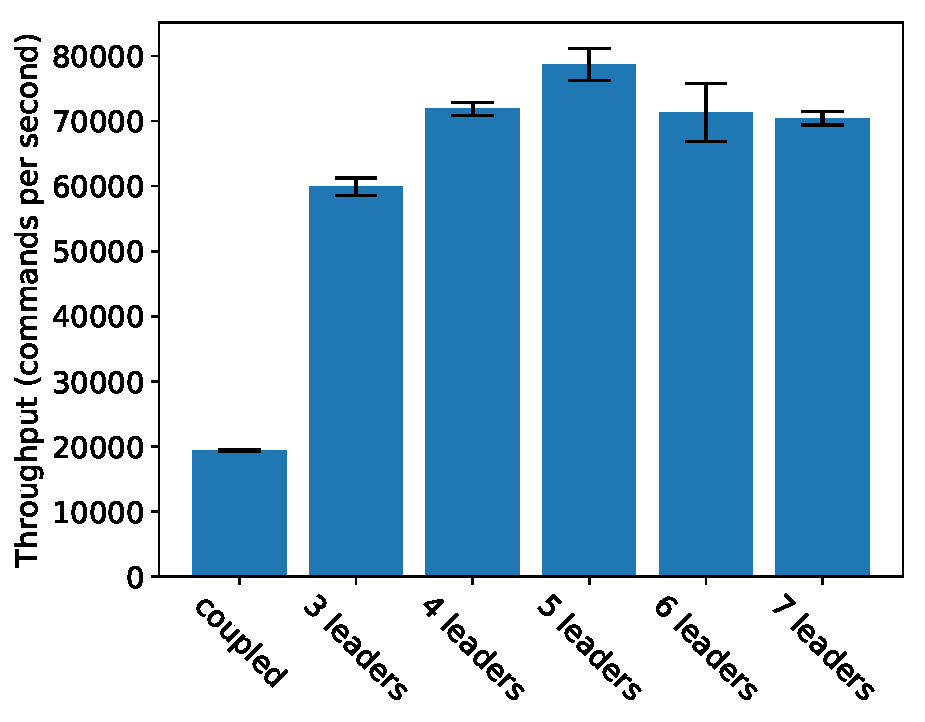
\includegraphics[width=\textwidth]{assets/nsdi_fig2_ablation_high_load_throughput.pdf}
    \caption{Throughput with 600 clients.}%
    \figlabel{EvalAblationHighLoadThroughput}
  \end{subfigure}\hspace{0.03\textwidth}
  \begin{subfigure}[b]{0.3\textwidth}
    \centering
    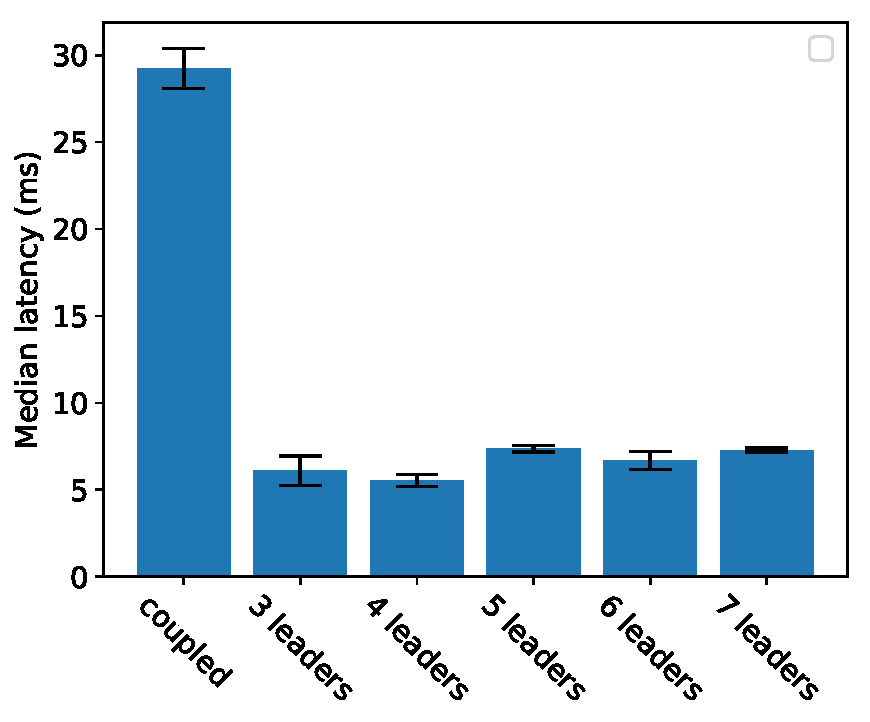
\includegraphics[width=\textwidth]{assets/nsdi_fig2_ablation_high_load_latency.pdf}
    \caption{Median latency (ms) with 600 clients.}%
    \figlabel{EvalAblationHighLoadLatency}
  \end{subfigure}\hspace{0.03\textwidth}
  \begin{subfigure}[b]{0.3\textwidth}
    \centering
    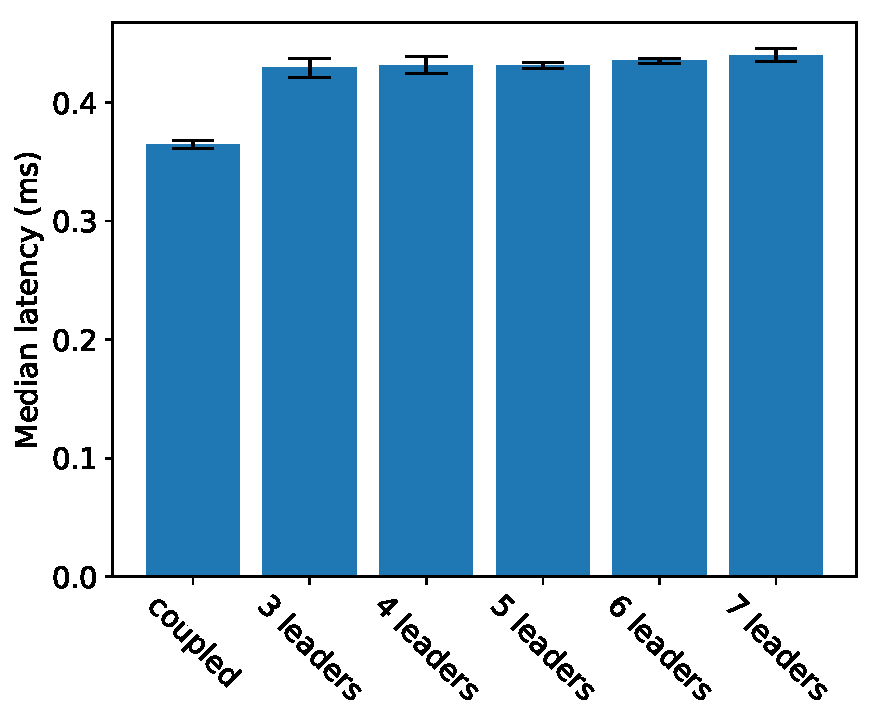
\includegraphics[width=\textwidth]{assets/nsdi_fig2_ablation_low_load_latency.pdf}
    \caption{Median latency (ms) with one client.}%
    \figlabel{EvalAblationLowLoadLatency}
  \end{subfigure}
  \caption{%
    An ablation study showing the effect of disaggregation and scaling on
    throughput and latency with 600 clients and one client. Throughput for one
    client is not shown because it is simply the inverse of latency.
  }\figlabel{EvalAblation}
\end{figure*}
}

\paragraph{Experiment Description.}
same setup as above
run all components in one proc
scale number of leaders
see effects of decoupling and scaling
high and low load

\paragraph{Results.}
under high load, 600 clients, coupled perofrms worse than multipaxos and epaxos
this is expected, bpaxos now has alot of orles
when we doucple, we see triplign in throughput, already beating state of the art
we scale up to 5 leaders to get an aditional 125\% throughput boost. once the leaders are not bottleneck, adding more doesnt help, it can acutallu hurt because more deps

latency is helped by decoupling but leaders doest affect latency much
at low load, the latency of coupled is slightly lower, fewer messages have to be sent across the network, this latency speedup would be even higher if we performened more aggresive forms of coupling

\subsection{Batching}
bpaxos modularity gives throughput wins at the cost of latency at low load. if we perform batching, we can trade off even more latnecy for significantly higher throughput. bpaxos super amenable to batching ebcause the overheads of receiving messages and forming batches fall on the eladers, which is scalable, acceptors and proposers run linear in batches, not commands, so amortized, larger batches, fewer vertices, faster graph traversal smaller and fewer cycles
give numbres too
